\documentclass[11pt,a4paper]{article}

\usepackage[margin=2.5cm]{geometry}
\usepackage[T1]{fontenc}
\usepackage{lmodern}
\usepackage{amsmath,amssymb}
\usepackage{booktabs}
\usepackage{graphicx}
\usepackage{array}
\usepackage{longtable}
\usepackage[hidelinks]{hyperref}

\newcommand{\ntests}{669}
\newcommand{\nchecks}{29}
\newcommand{\nbrowser}{3}
\newcommand{\nagree}{24}
\newcommand{\nexception}{4}
\newcommand{\nopen}{1}
\newcommand{\commit}{1bb3c37}


\setlength{\parindent}{0pt}
\setlength{\parskip}{0.6em}
\renewcommand{\arraystretch}{1.25}

\title{Verification of the score-based donation game engine}
\author{}
\date{18 October 2026}

\begin{document}
\maketitle

\section{Summary}

This report lists the checks made on the engine in \texttt{engine/}, the replicator-dynamics GUI in \texttt{gui/}, and the scripts that run on them. It covers the repository as built from commit \texttt{\commit} (the report and its figures are in \texttt{docs/verification/}). The notation is that of the notes \emph{Calculating the Stable Reputation Distribution in Infinite Population Models of Indirect Reciprocity}, which were read in full (pages 1--8).

\textbf{How to read it.} There are \nchecks{} checks, numbered 1 to \nchecks{}. Each says what was checked, what it was checked against, how many things were checked, and whether they agree. \emph{Agree} means that no difference was above what the check allows: rounding error for an exact calculation, sampling noise for the simulation. The report does not list the tolerances. \nagree{} checks agree, \nexception{} agree with an exception that is explained in the check, and \nopen{} is open (the two differ and the reason is not known).

\textbf{Two things to know.}
\begin{itemize}
\item The notes contain no ternary section, so the ternary results have no printed numbers to be compared with. Checks 10 to 19 check them against independent models, a simulation, closed forms and hand arithmetic instead.
\item Check~22 is the paper's published ESS table. The engine finds 359 of its 403 ESS and no others. The 44 it does not find are payoff ties (the invader's payoff is larger by at most $3.3\times10^{-16}$, so rounding decides). Running 200 steps does not come closer; the published file's header says 500 steps.
\end{itemize}

\begin{longtable}{@{}r>{\raggedright\arraybackslash}p{4.2cm}>{\raggedright\arraybackslash}p{4.6cm}>{\raggedright\arraybackslash}p{3.3cm}l@{}}
\toprule
\# & Kind of check & Checked against & How many & Result \\
\midrule
\endhead
1 & Binary engine & Julia code & 400 cases & Agree \\
2 & Binary ESS & Julia code & 3192 rows & Agree \\
3 & ESS sweep script & Julia code & 1296 norms $\times$ 2 noise levels & Agree \\
4 & Lifted ternary & binary engine & 12 cases and 1296 norms & Agree \\
5 & Notes: Defectors and Discriminators & the notes, pp.~5--6 & 7 quantities & Agree \\
6 & Notes: $\phi$-Disc rates & the notes, p.~7 & 5 + 1000 settings & Agree \\
7 & Notes: $\phi$-Disc, $\phi=1$ & the notes, p.~8 & 1 distribution, 6 settings & Agree \\
8 & Notes: $\phi=0$ & the notes & 500 settings & Agree \\
9 & Notes: stationary equations & the notes, Eq.~11 & 108 chains & Agree \\
10 & Independent model: rates & independent model & 5000 configurations & Agree \\
11 & Independent model: chains & independent model & 1780 chains & Agree \\
12 & Independent model: stationary & independent model & 227 + 107 settings & Agree \\
13 & Closed form: ternary & closed form & 100 configurations & Agree \\
14 & Mismatched classes & independent model & 2100 configurations & Agree \\
15 & Edge cases & independent model & 859 settings & Agree \\
16 & Drifting flag & the rule & 833 configurations & Agree* \\
17 & Agent-based simulation & simulation, $10^6$ agents & 470 comparisons & Agree* \\
18 & Hand-computed cases & hand arithmetic & 18 cases & Agree \\
19 & Planted bugs & 4 test suites & 25 planted bugs & Agree \\
20 & Leading Eight & the paper's code & 8 norms & Agree \\
21 & ESS figure & the paper's code & 2 figures, 20 tests & Agree \\
22 & Published ESS data & the paper's data & 403 ESS rows & Agree* \\
23 & Script: Markov chain & old script, committed runs & 20 + 1800 + 7 & Agree* \\
24 & Script: ESS sweep (old) & old script, Julia & 1296 norms & Agree \\
25 & Script: zeroness & old script, committed tables & 20736 chains & Agree* \\
26 & Replicator dynamics and rest points & games with known answers & 26 tests & Agree \\
27 & GUI & expected behaviour & 64 unit tests, 3 browser tests & Agree \\
28 & Saved results & the saved run & 26 tests & Agree \\
29 & Portability & Python 3.9 and 3.13 & 2 environments & Agree \\
\bottomrule
\end{longtable}
Agree = no difference above what the check allows (rounding error for exact calculations, sampling noise for the simulation). Agree* = agree, with an exception explained in the check. Open = they differ and it is not explained.


\section{The checks}

\subsection*{Check 1: Stable scores, payoffs and rates against the Julia code}
\addcontentsline{toc}{subsection}{Check 1: Stable scores, payoffs and rates against the Julia code}

\begin{description}\setlength\itemsep{0pt}

\item[What was checked] The engine's final score distributions, payoffs and the three rates $\alpha,\beta,\gamma$ of binary strategies and norms.

\item[Checked against] the output of \texttt{helper\_funcs.jl} (saved by \texttt{make\_reference.jl}).

\item[How many] 400 cases: 200 with one strategy and 200 with two, at noise 0, 0.01 and 0.1, run for 0 to 1000 steps.

\item[Result] \textbf{Agree}

\item[Note] Payoffs follow Julia's convention: one strategy from the distribution before the last step, two strategies from the final one.

\end{description}


\subsection*{Check 2: The ESS search against the Julia code}
\addcontentsline{toc}{subsection}{Check 2: The ESS search against the Julia code}

\begin{description}\setlength\itemsep{0pt}

\item[What was checked] The list of ESS that \texttt{find\_ESS} finds among the 16 binary strategies for a norm ($\rho_A=0.99$, 100 steps, fitness threshold $10^{-5}$).

\item[Checked against] the output of \texttt{helper\_funcs.jl} (saved by \texttt{make\_reference.jl}).

\item[How many] 3192 rows (1596 norms at noise 0 and at noise 0.01), 809 ESS in all.

\item[Result] \textbf{Agree}

\item[Note] Every row is compared by \texttt{tests/reference/compare\_ess.py}; the test suite checks a sample of 60.

\end{description}


\subsection*{Check 3: The sweep script against the Julia code}
\addcontentsline{toc}{subsection}{Check 3: The sweep script against the Julia code}

\begin{description}\setlength\itemsep{0pt}

\item[What was checked] The ESS found by the sweep script (the one that runs on R\=apoi).

\item[Checked against] The Julia ESS lists for the same norms.

\item[How many] 1296 CN-only binary norms at noise 0 and at noise 0.01.

\item[Result] \textbf{Agree}

\end{description}


\subsection*{Check 4: A ternary norm that ignores the cut-off against the binary result}
\addcontentsline{toc}{subsection}{Check 4: A ternary norm that ignores the cut-off against the binary result}

\begin{description}\setlength\itemsep{0pt}

\item[What was checked] A binary norm and binary strategies lifted to ternary classes must give exactly the binary results.

\item[Checked against] The binary engine.

\item[How many] 12 test cases (4 norms $\times$ $\tau\in\{1,2,5\}$), and an ESS sweep of the 1296 CN-only norms lifted to ternary.

\item[Result] \textbf{Agree}

\end{description}


\subsection*{Check 5: The worked example of pages 5 and 6}
\addcontentsline{toc}{subsection}{Check 5: The worked example of pages 5 and 6}

\begin{description}\setlength\itemsep{0pt}

\item[What was checked] The stationary distributions of Defectors and Discriminators at $\epsilon=0.1$, $\epsilon_\uparrow=0.4$, $\epsilon_\downarrow=0.6$, and the comparison of 2000 steps with them.

\item[Checked against] The closed-form numbers printed in the notes: $\pi_0=1/3$ and $0.754095$, $q(\boldsymbol\pi_0)=0.456286$, mean scores $0.326093$ and $2$, and the differences $1.10\times10^{-5}$ and $7.36\times10^{-5}$.

\item[How many] 7 quantities from the notes, and both distributions at scores 0 to 20.

\item[Result] \textbf{Agree}

\item[Note] The notes do not say how the 2000 steps start; the initial distribution $(0.5,0.5)$ reproduces their differences.

\end{description}

\begin{figure}[h]
\centering
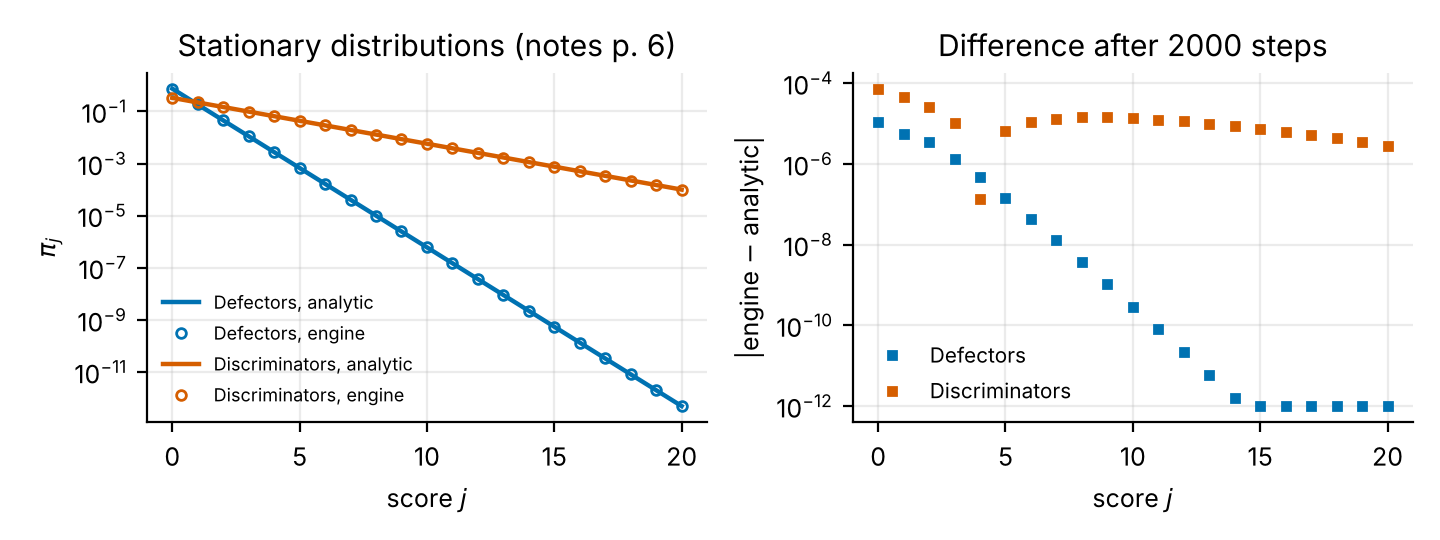
\includegraphics[width=\textwidth]{figures/defectors_discriminators.png}
\caption{Defectors and Discriminators. Left: closed-form stationary probabilities (lines) and the engine after 2000 steps (circles). Right: the absolute differences.}
\end{figure}


\subsection*{Check 6: The $\phi$-Disc rates of page 7}
\addcontentsline{toc}{subsection}{Check 6: The $\phi$-Disc rates of page 7}

\begin{description}\setlength\itemsep{0pt}

\item[What was checked] The up- and down-rates $g_j$ and $f_j$ of a population of $\phi$-Disc players under \texttt{CN:00000-0+ NC:00000000}.

\item[Checked against] The formulas of the notes, $G_j=\frac{1-w_0}{4(j-1)^{\phi}}$ and $F_j=\frac{1-w_0}{4}(1-j^{-\phi})$, with Eqs.~3--4.

\item[How many] 5 values of $\phi$ (0, 0.17, 0.5, 1, 2) at scores 1 to 7, and 1000 random settings ($\phi\in[0,3]$, noise, score distributions).

\item[Result] \textbf{Agree}

\item[Note] The notes print the norm as \texttt{CN:000000-+}, which is not a valid norm (a score-0 donor would lose a score); \texttt{CN:00000-0+} is meant and is what reproduces the notes' numbers.

\end{description}


\subsection*{Check 7: The $\phi=1$ stationary distribution of page 8}
\addcontentsline{toc}{subsection}{Check 7: The $\phi=1$ stationary distribution of page 8}

\begin{description}\setlength\itemsep{0pt}

\item[What was checked] The stationary score distribution of $\phi$-Disc players at $\epsilon=0.1$, $\epsilon_\uparrow=0.4$, $\epsilon_\downarrow=0.6$, and its $\pi_0$ and mean score.

\item[Checked against] The gamma-function solution of the notes ($\pi_0\approx0.2555$, $\mathbb{E}[\text{score}]=1.889$), with $\pi_0$ from the normalisation equation.

\item[How many] 1 distribution at all 440 tracked scores; 6 further settings of the noise.

\item[Result] \textbf{Agree}

\end{description}

\begin{figure}[h]
\centering
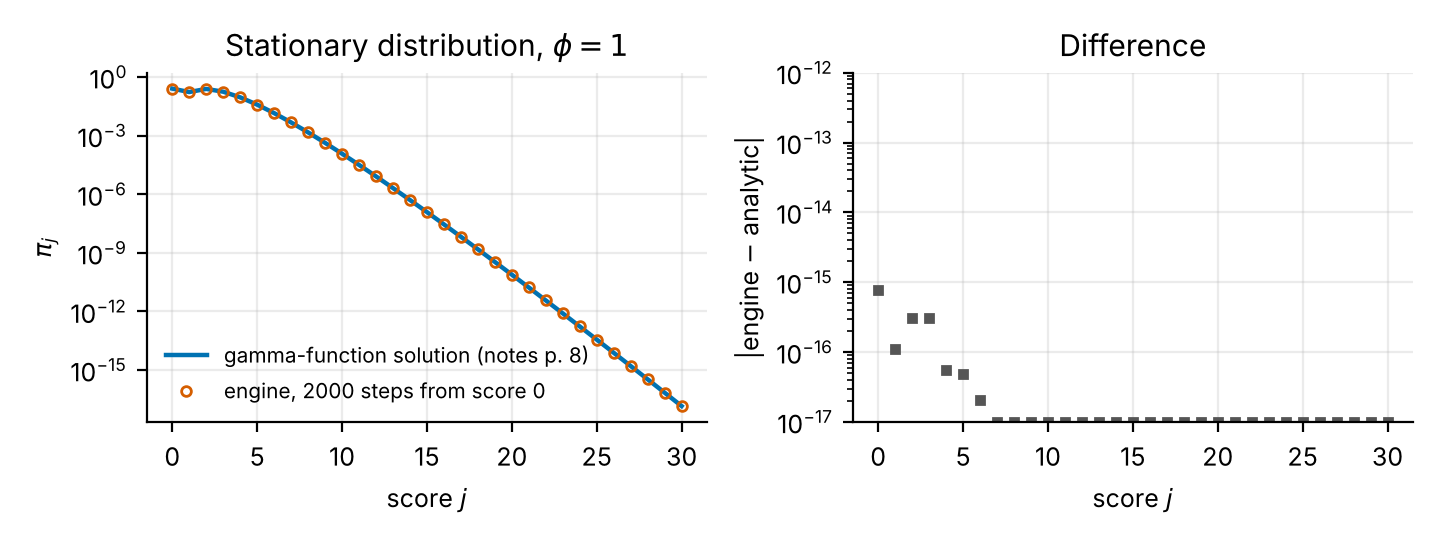
\includegraphics[width=\textwidth]{figures/phi_disc.png}
\caption{$\phi$-Disc with $\phi=1$. Left: the gamma-function solution (line) and the engine after 2000 steps from score 0 (circles). Right: the absolute differences.}
\end{figure}


\subsection*{Check 8: $\phi=0$ is the Discriminators}
\addcontentsline{toc}{subsection}{Check 8: $\phi=0$ is the Discriminators}

\begin{description}\setlength\itemsep{0pt}

\item[What was checked] The rates of $\phi$-Disc with $\phi=0$ and of Discriminators in the same population.

\item[Checked against] Each other (the notes say the two coincide).

\item[How many] 500 random settings of the norm, noise and score distribution.

\item[Result] \textbf{Agree}

\end{description}


\subsection*{Check 9: The fixed-point equation for $\pi_0$ (Eq.~11)}
\addcontentsline{toc}{subsection}{Check 9: The fixed-point equation for $\pi_0$ (Eq.~11)}

\begin{description}\setlength\itemsep{0pt}

\item[What was checked] $\pi_0=\dfrac{f-g}{f-g+g_1}$ evaluated at the engine's converged distribution.

\item[Checked against] The engine's own $\pi_0$.

\item[How many] 108 chains from 150 random binary settings with one or two strategies (the 73 settings that never settled within 4000 steps were left out).

\item[Result] \textbf{Agree}

\item[Note] The detailed-balance equations (Eqs.~5--6) are checked on the stationary distributions in Check~12.

\end{description}


\subsection*{Check 10: The rates $G,F,g,f$ against an independent implementation}
\addcontentsline{toc}{subsection}{Check 10: The rates $G,F,g,f$ against an independent implementation}

\begin{description}\setlength\itemsep{0pt}

\item[What was checked] The transition rates for random populations of binary, ternary and $\phi$-Disc strategies.

\item[Checked against] an independent re-implementation of the model written from the notes and \texttt{helper\_funcs.jl} without looking at the engine's code (\texttt{tests/independent\_model.py}).

\item[How many] 5000 random configurations: binary, ternary and lifted norms; $\tau\in\{1,2,3,5,8\}$; one to three strategies of mixed kinds (probabilistic and deterministic tables, $\phi\in[0,3]$); noise from 0 to 1; shares of zero; score distributions with mass beyond $\tau$.

\item[Result] \textbf{Agree}

\end{description}


\subsection*{Check 11: The score chains over time against the independent implementation}
\addcontentsline{toc}{subsection}{Check 11: The score chains over time against the independent implementation}

\begin{description}\setlength\itemsep{0pt}

\item[What was checked] The score distributions after 25 to 400 steps of the chain, with mass conserved.

\item[Checked against] The independent implementation iterating the same chain.

\item[How many] 1780 chains.

\item[Result] \textbf{Agree}

\end{description}


\subsection*{Check 12: Stationary distributions}
\addcontentsline{toc}{subsection}{Check 12: Stationary distributions}

\begin{description}\setlength\itemsep{0pt}

\item[What was checked] Whether a stationary distribution found independently (Eqs.~5--6 and a fixed point on the class masses) is left unchanged by one engine step, and whether the engine's own converged runs reach it.

\item[Checked against] The independent implementation.

\item[How many] 227 random settings for the first, 107 for the second.

\item[Result] \textbf{Agree}

\item[Note] How close a converged run gets is set by the engine's stopping rule, not by the model.

\end{description}


\subsection*{Check 13: Three geometric segments for a class-based ternary strategy}
\addcontentsline{toc}{subsection}{Check 13: Three geometric segments for a class-based ternary strategy}

\begin{description}\setlength\itemsep{0pt}

\item[What was checked] The stationary distribution of one ternary strategy, which is geometric over the three classes.

\item[Checked against] The closed form, with the class masses solved self-consistently, independently of the engine.

\item[How many] 100 configurations ($\tau\in\{1,2,3,5,8\}$).

\item[Result] \textbf{Agree}

\end{description}


\subsection*{Check 14: Strategies whose classes differ from the norm's}
\addcontentsline{toc}{subsection}{Check 14: Strategies whose classes differ from the norm's}

\begin{description}\setlength\itemsep{0pt}

\item[What was checked] Rates when a strategy's cut-off $\tau$ differs from the norm's, or a binary strategy meets a ternary norm and the other way round (the engine uses the raw scores).

\item[Checked against] The independent implementation.

\item[How many] 2100 configurations.

\item[Result] \textbf{Agree}

\end{description}


\subsection*{Check 15: Awkward settings}
\addcontentsline{toc}{subsection}{Check 15: Awkward settings}

\begin{description}\setlength\itemsep{0pt}

\item[What was checked] Rates and chains at $\tau=1$, with an empty top class, with $\epsilon=0$, and with a strategy whose share is 0.

\item[Checked against] The independent implementation (a population with and without the strategy of share 0).

\item[How many] $\tau=1$: 300; empty top class: 200; $\epsilon=0$: 159; share 0: 200.

\item[Result] \textbf{Agree}

\end{description}


\subsection*{Check 16: Which chains are flagged as drifting}
\addcontentsline{toc}{subsection}{Check 16: Which chains are flagged as drifting}

\begin{description}\setlength\itemsep{0pt}

\item[What was checked] That the engine flags a chain exactly when its up-rate at the top score is positive and at least its down-rate.

\item[Checked against] The rule, evaluated independently.

\item[How many] 833 configurations.

\item[Result] \textbf{Agree} (with the exception below)

\item[Note] When nothing can move (both rates 0) the engine does not flag the chain; the README now says so.

\end{description}


\subsection*{Check 17: A simulated population against the engine}
\addcontentsline{toc}{subsection}{Check 17: A simulated population against the engine}

\begin{description}\setlength\itemsep{0pt}

\item[What was checked] Score histograms after the same number of steps: a population of $10^6$ agents meeting random partners, with roles, help, the norm and noise drawn as in the model, against the engine.

\item[Checked against] The engine, bin by bin, with binomial standard errors.

\item[How many] 470 comparisons (the two example runs, $\phi$-Disc alone, Defectors against Discriminators, random ternary norms, a mix of $\phi$-Disc and a ternary strategy); 11 stationary scenarios, 48 comparisons.

\item[Result] \textbf{Agree} (with the exception below)

\item[Note] Two comparisons, both in one random case that the engine flags as drifting, fall outside the noise: the default stopping tolerance leaves the engine short of the stationary law there. The same test detects a 10\% error in $\epsilon$ and a 4\% error in the role factor.

\end{description}


\subsection*{Check 18: Small cases worked out on paper}
\addcontentsline{toc}{subsection}{Check 18: Small cases worked out on paper}

\begin{description}\setlength\itemsep{0pt}

\item[What was checked] Rates for tiny populations at $\tau=1$ and $2$: CN against NC, the recipient's index against the donor's, the class boundary at scores $\tau$ and $\tau+1$, the noise arithmetic, the $\phi$-Disc exponent, one step of the chain.

\item[Checked against] Numbers written as literal arithmetic from the notes.

\item[How many] 18 cases.

\item[Result] \textbf{Agree}

\end{description}


\subsection*{Check 19: Would the checks notice a mistake?}
\addcontentsline{toc}{subsection}{Check 19: Would the checks notice a mistake?}

\begin{description}\setlength\itemsep{0pt}

\item[What was checked] Whether the test suites fail when a bug is planted in a copy of the engine (a wrong cut-off, a swapped CN and NC, a transposed table, a wrong lift to ternary, the wrong score in the $\phi$ exponent, a wrong role factor, \dots).

\item[Checked against] Four suites: the hand cases, the independent tests, the repository's own tests and the simulation tests.

\item[How many] 25 planted bugs.

\item[Result] \textbf{Agree}

\item[Note] Every bug was caught by at least one suite. No single suite caught them all (the repository's own tests missed three cut-off bugs; the simulation tests missed a transposed table and a wrong lift), which is why all four are kept.

\end{description}


\subsection*{Check 20: The Leading Eight norms}
\addcontentsline{toc}{subsection}{Check 20: The Leading Eight norms}

\begin{description}\setlength\itemsep{0pt}

\item[What was checked] The barcodes, names and ESS strategies of L1 to L8 in \texttt{known\_norms.py}, and whether the engine finds a fully cooperative ESS for each.

\item[Checked against] \texttt{createLeading8()} in the paper's code, and the engine's own ESS search (noise 0.001 and 0.01).

\item[How many] 8 norms: barcodes and strategies equal; a cooperative ESS found for 8 of 8.

\item[Result] \textbf{Agree}

\item[Note] The five entries all eight share and the three that vary are also checked in the tests.

\end{description}


\subsection*{Check 21: The ESS figure against the paper's}
\addcontentsline{toc}{subsection}{Check 21: The ESS figure against the paper's}

\begin{description}\setlength\itemsep{0pt}

\item[What was checked] \texttt{plots/ess\_plot.py}: the layout, sort order, cell widths, colours and Leading Eight labelling.

\item[Checked against] The paper's \texttt{plotting\_funcs.py} and the figures it produced.

\item[How many] 2 data files drawn and compared by eye (25 and 403 rows), and 20 unit tests.

\item[Result] \textbf{Agree}

\end{description}


\subsection*{Check 22: The paper's published ESS table}
\addcontentsline{toc}{subsection}{Check 22: The paper's published ESS table}

\begin{description}\setlength\itemsep{0pt}

\item[What was checked] The ESS the engine finds for every CN-only norm (1296) at noise 0.01, 500 steps and the paper's fitness threshold 0.01, compared by norm and strategy, and their cooperation levels.

\item[Checked against] The paper's file \texttt{tokens\_CmeetsN\_Noise0.01\_B2} (its header says 500 steps).

\item[How many] 403 published ESS rows (302 norms); the same sweep with 200 and 100 steps.

\item[Result] \textbf{Agree} (with the exception below)

\item[Note] The engine finds 359 of the 403 and no ESS that the file lacks; the cooperation levels of the 359 differ by at most $8\times10^{-4}$. The other 44 (in 25 norms) are payoff ties: the invader's payoff is larger than the resident's by at most $3.3\times10^{-16}$, because strategies that differ only where it never matters earn the same payoff and rounding decides. Running 200 steps does not come closer: it finds 362 but adds 33 ESS that the file lacks and the cooperation levels differ by up to 0.27 (100 steps: 346 found, 29 extra, up to 0.45). The file's header says 500 steps.

\end{description}


\subsection*{Check 23: \texttt{run\_markov\_chain.py} on the engine}
\addcontentsline{toc}{subsection}{Check 23: \texttt{run\_markov\_chain.py} on the engine}

\begin{description}\setlength\itemsep{0pt}

\item[What was checked] Rates, class masses and score distributions of every step, and the number of steps.

\item[Checked against] The old script and the seven run directories committed in the repository.

\item[How many] 20 argument sets, 1800 random norms, strategies and initial distributions, and 7 committed runs.

\item[Result] \textbf{Agree} (with the exception below)

\item[Note] The old script capped scores at \texttt{maxw}; the engine does not. Where the cap did not bind the two agree. Where it did, the rates and class masses still agree in the committed runs while the score distributions continue above the cap; with a very small cap the old results differ.

\end{description}


\subsection*{Check 24: \texttt{experiments/ESS/find\_ESS\_parellel.py} on the engine}
\addcontentsline{toc}{subsection}{Check 24: \texttt{experiments/ESS/find\_ESS\_parellel.py} on the engine}

\begin{description}\setlength\itemsep{0pt}

\item[What was checked] The ESS found for every CN-only norm, and the CSV written.

\item[Checked against] The old code, the committed CSV and the Julia ESS lists.

\item[How many] 1296 norms (333 ESS rows); the ternary path in 64 cases.

\item[Result] \textbf{Agree}

\item[Note] The old code took two-strategy payoffs from the distribution before the last step and the engine, like Julia, from the final one; this only reorders near-ties and changes no ESS.

\end{description}


\subsection*{Check 25: \texttt{experiments/verify-zeroness-one-strategy} on the engine}
\addcontentsline{toc}{subsection}{Check 25: \texttt{experiments/verify-zeroness-one-strategy} on the engine}

\begin{description}\setlength\itemsep{0pt}

\item[What was checked] The group of initial rates, the final rates and the share of score 0 of every chain, and the limit-check tables.

\item[Checked against] The old code and the committed tables.

\item[How many] 20736 chains (1296 norms $\times$ 16 strategies); the 20736-row limit-check table; the rate function at 11 class masses for every chain.

\item[Result] \textbf{Agree} (with the exception below)

\item[Note] The old chains were capped at \texttt{maxw}, so about half of them now track more scores; the limit check keeps its own capped chain.

\end{description}


\subsection*{Check 26: Games with known answers}
\addcontentsline{toc}{subsection}{Check 26: Games with known answers}

\begin{description}\setlength\itemsep{0pt}

\item[What was checked] Rest points and their stability, the replicator equation, and the restart of the score chains.

\item[Checked against] Games whose answers are known (prisoner's dilemma, hawk--dove, coordination with two and three strategies, rock--paper--scissors in both versions), the invasion fitness of the engine's own payoffs, and the analytic Cooperators against Defectors.

\item[How many] 26 tests (19 for the simplex and rest points, 7 for the dynamics).

\item[Result] \textbf{Agree}

\end{description}


\subsection*{Check 27: The GUI logic and a click-through in a browser}
\addcontentsline{toc}{subsection}{Check 27: The GUI logic and a click-through in a browser}

\begin{description}\setlength\itemsep{0pt}

\item[What was checked] Input checks, settings files, presets, figures, the strategies and norm cards, and a click through all three pages in Chromium (including going back to the results, typing axis ranges and saving).

\item[Checked against] The expected behaviour.

\item[How many] 64 unit tests, and 3 browser tests (full click-through, two strategies from a settings file, save and load).

\item[Result] \textbf{Agree}

\end{description}


\subsection*{Check 28: Saving a result and loading it again}
\addcontentsline{toc}{subsection}{Check 28: Saving a result and loading it again}

\begin{description}\setlength\itemsep{0pt}

\item[What was checked] That a loaded result has every number of the saved one, that a new point can still be computed, that the file is plain queryable tables, and that a taken name, a damaged file and a foreign file are refused.

\item[Checked against] The finished run that was saved (2 and 3 strategies).

\item[How many] 26 tests; every point on the simplex, every trajectory step, every matrix and distribution.

\item[Result] \textbf{Agree}

\item[Note] The far tail of each score distribution (probabilities below $10^{-12}$) is not stored and reads back as 0.

\end{description}


\subsection*{Check 29: Other versions of Python}
\addcontentsline{toc}{subsection}{Check 29: Other versions of Python}

\begin{description}\setlength\itemsep{0pt}

\item[What was checked] That the engine and the sweep run on the Python that R\=apoi provides.

\item[Checked against] Python 3.9 with numpy 1.26 and scipy 1.11, and Python 3.13 with numpy 2.5 and scipy 1.18.

\item[How many] 2 environments: 517 engine tests and the sweep tests on 3.9; the whole suite on 3.13.

\item[Result] \textbf{Agree}

\end{description}



\section{Tests in the repository}

\texttt{python -m pytest} runs \ntests{} tests, all passing; \nbrowser{} browser tests (\texttt{-m e2e}, Chromium through Playwright) are run separately and also pass. Many of the checks above are in the suite, so they run every time.

\begin{center}
\begin{tabular}{@{}lrl@{}}
\toprule
File & Tests & Covers \\
\midrule
\texttt{test\_against\_julia.py} & 460 & 400 stable-score cases, 60 sampled ESS rows \\
\texttt{test\_engine.py} & 32 & norms, strategies, closed forms, invariants \\
\texttt{test\_independent\_model.py} & 19 & independent re-implementation \\
\texttt{test\_agent\_based.py} & 12 & agent-based simulation \\
\texttt{test\_hand\_cases.py} & 1 & 18 hand-computed cases \\
\texttt{test\_simplex.py} & 19 & grid, rest points, stability \\
\texttt{test\_replicator.py} & 7 & dynamics, restart, role factor \\
\texttt{test\_known\_norms.py} & 12 & Leading Eight \\
\texttt{test\_plots.py} & 20 & ESS figure and readers \\
\texttt{test\_saves.py} & 18 & saving and loading results \\
\texttt{test\_gui\_logic.py} & 55 & GUI logic \\
\texttt{test\_ess\_sweep.py} & 6 & ESS sweep script \\
\texttt{test\_experiments.py} & 4 & migrated experiment scripts \\
\texttt{test\_run\_markov\_chain.py} & 4 & Markov chain script \\
\midrule
Total & 669 & \\
\bottomrule
\end{tabular}

\end{center}

\section{What has not been verified}

\begin{itemize}
\item The conventions for ternary strategies and norms (the cut-off at $\tau$, the order of the 18 characters of a barcode, the orientation of a strategy table) are not printed in the notes. They rest on the description given for the engine and on the lifting identity (Check~4); the independent models share them with the engine.
\item The notes give a closed form for $\phi$-Disc only at $\phi=1$. For other $\phi$ the engine agrees with the rates in the notes, but no stationary distribution has been compared with a closed form.
\item The role factor $q(1-q)$ is tested against its definition and by scaling, but Julia only ever uses $q=1/2$.
\item The replicator dynamics, the rest-point classification and the GUI have no reference implementation; they rest on games with known answers and on the tests above.
\item Results at the default tolerance ($10^{-5}$ on the change in one step) are approximate for slowly relaxing chains, in the engine and in the Julia code alike. A chain flagged as drifting has no stable distribution at the rates it has at the top score, but one can exist for other class masses, and the chain can take very long to reach it.
\item Payoffs and the ESS search were checked against Julia for binary strategies only; for ternary strategies the independent checks cover rates, chains and stationary distributions, not the ESS search.
\item The Slurm scripts in \texttt{scripts/raapoi/} have been tested locally, with the Slurm environment variables set by hand, but have not been run on R\=apoi itself.
\end{itemize}

\section{Reproducing the checks}

\begin{verbatim}
python -m pytest                          # the tests above
python -m pytest -m e2e                   # browser tests (needs playwright)
python tests/reference/compare_ess.py     # every ESS row against Julia
PYTHONPATH=. python docs/verification/make_figures.py   # the two figures
python docs/verification/build_report.py  # the checks of this report
\end{verbatim}

\end{document}
